\documentclass{beamer}

\usepackage{babel}
\usepackage{tikz}
%\usetheme{boxes}
\usepackage[utf8]{inputenc}
\usepackage{amsmath}
\usepackage{amsthm}
\usepackage{hyperref}
\usepackage{natbib}
\usepackage{tikz}
\usepackage{xcolor}
\usepackage[absolute,overlay]{textpos}
\bibliographystyle{plainnat}
\usecolortheme{crane}

\definecolor{orange}{RGB}{232, 86, 15}
\definecolor{blue}{RGB}{14, 159, 232}
\definecolor{blueblue}{RGB}{50, 90, 160}
\definecolor{yellow}{RGB}{232, 187, 14} 
\definecolor{red}{RGB}{232, 14, 59}
\newtheorem{deff}{Definición}
%Information to be included in the title page:
\institute[]{}

\setbeamercolor{title}{bg=blueblue, fg=white}
\setbeamercolor{subttile}{bg=blueblue, fg=white}
\setbeamercolor{frametitle}{bg=blueblue, fg=white}
\setbeamercolor{block title}{bg=blue, fg=white}
\setbeamercolor{block title alerted}{bg=red, fg=white}
\setbeamercolor{block title example}{bg=yellow, fg=white}
\setbeamercolor{footline}{bg=gray, fg=white}
\beamertemplatenavigationsymbolsempty

	
\newcommand{\indep}{\perp \!\!\! \perp}

\newcommand\blfootnote[1]{%
  \begingroup
  \renewcommand\thefootnote{}\footnote{#1}%
  \addtocounter{footnote}{-1}%
  \endgroup
}


\newcommand\overalert[2]{
	 \only<#1>{
\begin{textblock*}{\textwidth}(.35\textwidth,0.25\textheight)
    \begin{beamercolorbox}[wd=.5\textwidth,center,sep=0.3cm]{block title alerted}
	    #2
    \end{beamercolorbox}
\end{textblock*}
}
}

\newcommand\overexample[2]{
	 \only<#1>{
\begin{textblock*}{\textwidth}(.35\textwidth,0.25\textheight)
    \begin{beamercolorbox}[wd=.5\textwidth,center,sep=0.3cm]{block title example}
	    #2
    \end{beamercolorbox}
\end{textblock*}
}
}


\newcommand\overeblock[2]{
	 \only<#1>{
\begin{textblock*}{\textwidth}(.35\textwidth,0.25\textheight)
    \begin{beamercolorbox}[wd=.5\textwidth,center,sep=0.3cm]{block title}
	    #2
    \end{beamercolorbox}
\end{textblock*}
}
}

\title{Causal frameworks and framing causal problems}
\author{Gherardo Varando}
\date{IPL \\ 04 May 2023}
\begin{document}

\begin{frame}
	\titlepage
\end{frame}

\begin{frame}{Summary of last session}
	\begin{columns}
		\begin{column}{0.5\textwidth}
	\begin{itemize}
		\item statistical models
		\item BN/DAG, d-separation and conditional independences 
	\end{itemize}
		\end{column}
		\begin{column}{0.5\textwidth}
			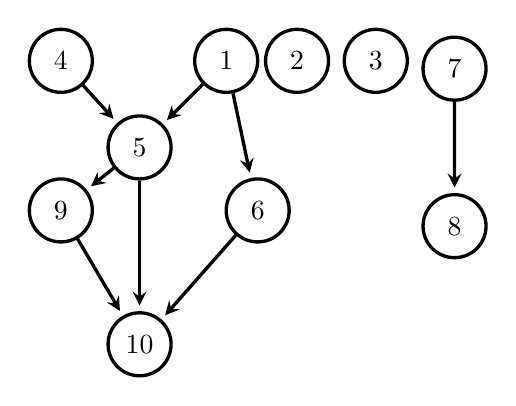
\begin{tikzpicture}[scale=5, 
       node/.style={circle,inner sep=1mm,minimum size=0.8cm,draw,
      very thick,black,fill=white,text=black},
        nondirectional/.style={very thick,black},
        unidirectional/.style={nondirectional,shorten >=2pt,-stealth},
        bidirectional/.style={unidirectional,bend right=10}]

	\node [node] (v1) at (0.420000, 0.720000)       {1};
        \node [node] (v2) at (0.60000, 0.720000)        {2};
        \node [node] (v3) at (0.80000, 0.720000)        {3};
        \node [node] (v4) at (0.00000, 0.720000)        {4};
        \node [node] (v5) at (0.200000, 0.500000)       {5};
        \node [node] (v6) at (0.500000, 0.340000)       {6};
        \node [node] (v7) at (1.000000, 0.700000)       {7};
        \node [node] (v8) at (1.000000, 0.300000)       {8};
        \node [node] (v9) at (0.00000, 0.340000)        {9};
	\node [node] (v10) at (0.200000, 0.000000)      {10};

        \path [unidirectional] (v1) edge (v5);
        \path [unidirectional] (v4) edge (v5);
        \path [unidirectional] (v5) edge (v9);
        \path [unidirectional] (v5) edge (v10);
        \path [unidirectional] (v1) edge (v6);
        \path [unidirectional] (v6) edge (v10);
        \path [unidirectional] (v7) edge (v8);
        \path [unidirectional] (v9) edge (v10);
\end{tikzpicture}

		\end{column}
	\end{columns}
\end{frame}

\begin{frame}{Causal models desiderata}
	\begin{itemize}
		\item Represent data, similar to a statistical model 
		\item Model what happen when changes/experiment/interventions  
		\item Reason on and explore the causal relationships 
		\item Represent causal relationships 
	\end{itemize}
\end{frame}

\begin{frame}{Causal regression models}
      \begin{itemize}
	      \item given a regression model $Y = f(X, \varepsilon)$ 
		      we could interpret this as a causal model 
	      \item in the sense that we imagine the physical/true generating process 
		      to be modeled by this equation 
	      \item<2-> If we make \emph{experiments} by changing the value of $X$ we know that 
		      the associated value for $Y$ is generated accordingly to $f(X, \varepsilon)$ 
      \end{itemize}
\end{frame}

\begin{frame}{Structural Causal Models}
	\begin{block}{Definition \citep{peters2017elements}}
 A SCM over variables $X_1, \ldots, X_p$ with noise variables $\varepsilon_1, \ldots, \varepsilon_p$ is 
	 a collection of \textbf{structural assignments}: 
	   \[ X_i =  f_i(X_{pa(i)}, \varepsilon_i) \]
	   where $\varepsilon_i$ are assumed jointly independent and $f_i$ are fixed deterministic functions.  
	 \end{block}
	 \begin{itemize}
		 \item $X_{pa(i)}$ are called the parents or the \textbf{direct causes} of $X_i$
		 \item we say $X_i$ is a direct effect of its direct causes 
		 \item we assume the associated graph $G$ to be a DAG 
		 \item<2-> A SCM defines a unique distribution $P$ over the variables $X_1, \ldots, X_p$ 
		 \item<3-> $(G, P)$ is a Bayesian network 
	 \end{itemize}
	 \blfootnote{\citet{bareinboim2022pearl}}
\end{frame}


\begin{frame}{Interventions in SCM}
	\begin{itemize}
		\item given a SCM we define an experiment, or intervention when we \textbf{replace one or several of the structural assignments} to obtain a new SCM
		\item<2-> the interventional distribution under this change is the new entailed probability distribution defined by the new SCM
		\item<3-> e.g if changing one of the assignment (for $X_k$) we can write $P^{do(X_k = \tilde{f}_k(X_{\tilde{pa}(k)}, \tilde{\varepsilon}))}$ the new interventional distribution 
		\item<3-> sometimes you can find $P(\cdot| do())$ 
		\item<4-> we say there is a \textbf{total causal effect} from $X$ to $Y$ in a SCM 
			if and only if there exist a random variable $\tilde{N}$ such that 
			\[ X \not \indep Y \text{ in } P^{do(X = \tilde{N})} \]
	\end{itemize}
\end{frame}

\begin{frame}
	\begin{itemize}
		\item SCM defines an \textbf{observational distribution} plus \textbf{interventional distributions} for each of the possible interventions 
		\item The set of observational and interventional distributions can also be represented with a Causal BN 
		\item<2-> but SCMs allow an additional causal reasoning step: \textbf{counterfactuals}  
	\end{itemize}
\end{frame}

\begin{frame}{Counterfactual statements}
	\begin{itemize}
		\item<1-> Given some observed state/event,what would have happened if ... ? 
		\item<2-> I have headache, I take aspirin and one hour later the pain disappear. 
		      Would the pain had disappeared if I had not taken aspirin? 
	      \item<3-> this is different from interventions since we are not just doing an experiment, 
		      but rather imagining interventions for alternative \emph{worlds}, that is 
			alternative ways the system could have evolved but conditioning on everything 
			else being the same 
	\end{itemize}
\end{frame}

\begin{frame}{Counterfactuals in SCM}
	\begin{itemize}
		\item SCMs allow the computation of counterfactual probabilities 
		\item Counterfactual statements can be seen as intervention/do-statements in 
			a counterfactual SCM which is obtained from an initial SCM by replacing the 
			noise distribution with $P(\varepsilon | X = x)$
		\item<2-> SCM can induce same observational and interventional distribution (Causal BN) 
			but different counterfactuals
	\end{itemize}
	\blfootnote{\citet{peters2017elements, bareinboim2022pearl}}

\end{frame}

\begin{frame}{Example from \citet{peters2017elements}}
	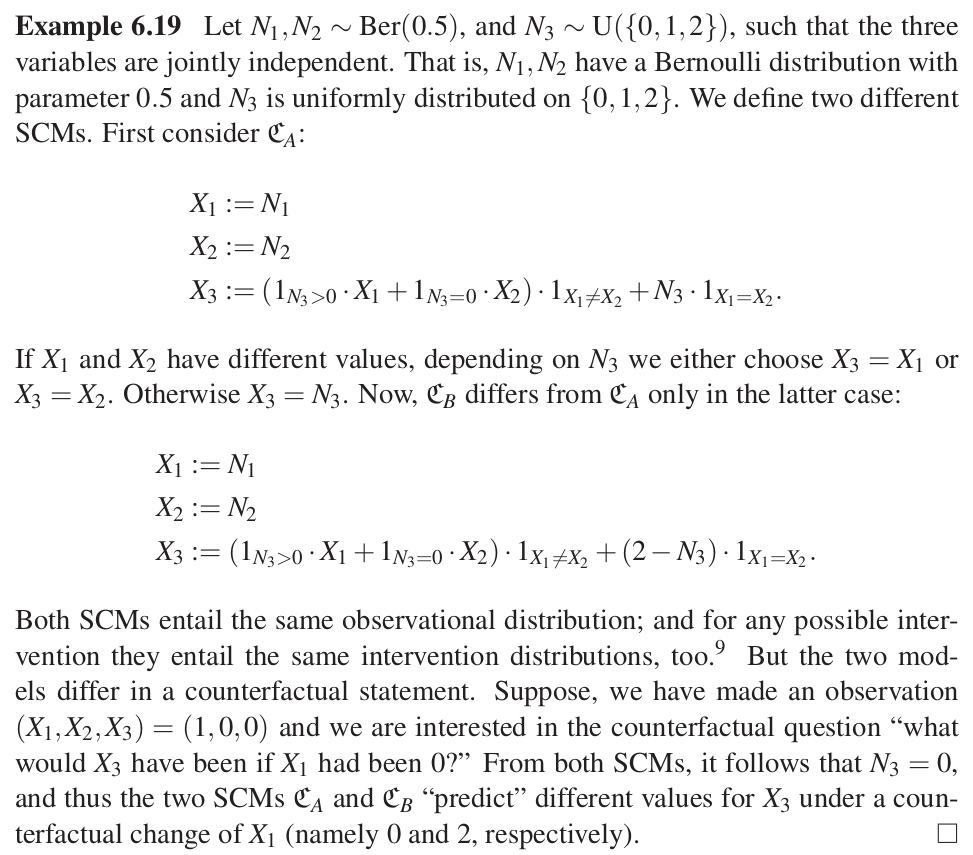
\includegraphics[scale=0.25]{images/counter_example}
\end{frame}

\begin{frame}{Pearl Causal Hierarchy (PCH)}
	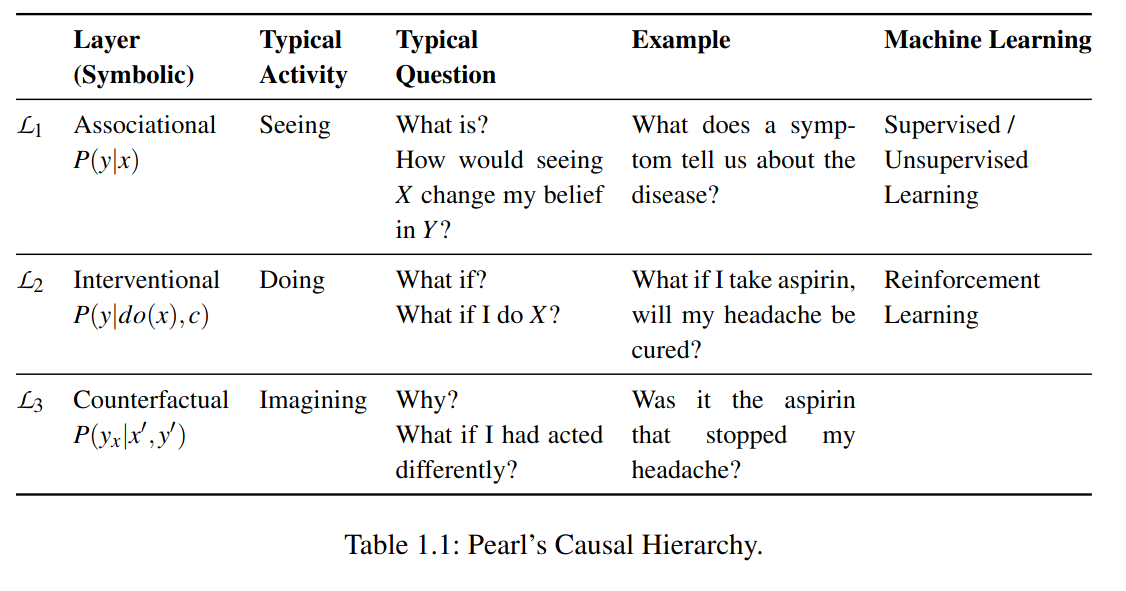
\includegraphics[scale=0.3]{images/PCH} 
	\blfootnote{\citet{bareinboim2022pearl}}
\end{frame}

\begin{frame}{Potential outcomes - Counterfactual model}
	\begin{itemize}
		\item consider a binary \textbf{treatment variable} $A$ (1: treated, 0: untreated)    
		\item and a binary \textbf{outcome} $Y$ (1: death, 0: survival) 
		\item $A,Y$ are random variables that take possible different values for each individual
		\item<2-> denote with $Y^{a=1}$ (Y under treatment $a=1$) the outcome variable that would have been observed under treatment $a=1$, and similarly $Y^{a=0}$ 
		\item<2-> $Y^{a=1}$ and $Y^{a=0}$ are called \textbf{potential outcomes} or \textbf{counterfactual outcomes} 
		\item<3-> for each individual, only one of the potential outcomes 
			if actually observed/factual. 
			\[ Y = Y^{a=A}  \quad \text{(consistency equation)} \]
	\end{itemize}
	\blfootnote{\citet{whatif, wasserman2004all}}

\end{frame}

\begin{frame}{Causal effects}
	\begin{definition}{Individual causal effects}
The treatment $A$ has a causal effect on an individual's outcome $Y$ if $Y^{a=1} \neq Y^{a=0}$ 
	\end{definition}

	\begin{definition}{Average causal effects}
		An average causal effect of treatment $A$ on outcome $Y$ is present if 
		\[ P(Y^{a=1} = 1) \neq   P(Y^{a=0} = 1) \]
	\end{definition}
\end{frame}

\begin{frame}{Other causal frameworks}
	\begin{itemize}
		\item<1-> Granger causality
		\item<2-> Causal interpretation of dynamical system, ODE and SDE \citep{mooij2013ordinary, peters2022causal, hansen2014causal} 
		\item<3-> Cyclic causal models~\citep{hyttinen2012learning, bongers2016theoretical}    
		\item<4-> Equilibrium models~\citep{young2019identifying, varando2020graphical}
		\item<5-> Dynamic Causal Models (DCM)~\citep{friston2003dynamic}
		\item<6-> Local Independence Graphs~\citep{didelez2006asymmetric, mogensen2020markov}  
	\end{itemize}
\end{frame}


\begin{frame}{Causal problems}
\begin{itemize}
	\item<1-> Discovering causal relationships  (causal discovery) 
	\item<2-> Estimating causal effects (causal inference) 
	\item<3->  Exploiting causal information in ML/prediction/forecasting/RL 
\end{itemize}
\end{frame}


\begin{frame}{Causal Discovery} 
	\begin{columns}
		\begin{column}{0.5\textwidth}
			\begin{itemize}
				\item<1-> Which are the regions most affected by ENSO? 
				\item<2-> Which are the causal drivers and the causal 
					relationships involving food insecurity? 
				\item<3-> Retrieve the reaction network between genes and proteins from single-cell data 
			\end{itemize}
		\end{column}
		\begin{column}{0.5\textwidth}
			\only<1>{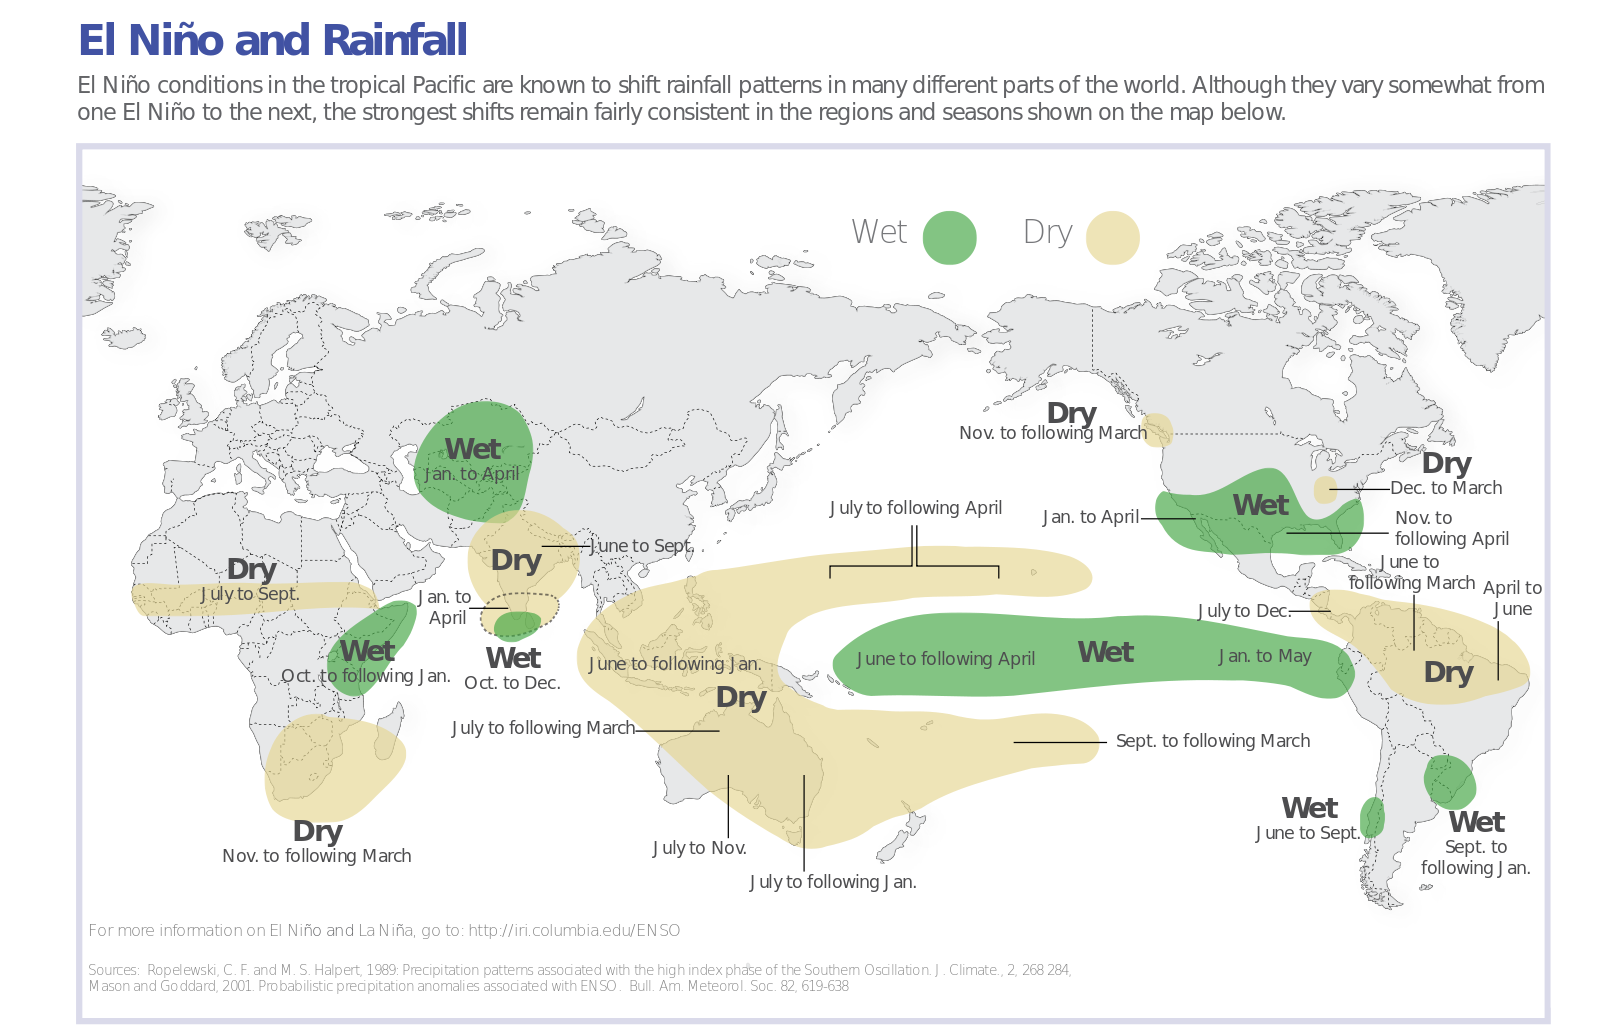
\includegraphics[scale=0.1]{images/enso}}
			\only<2>{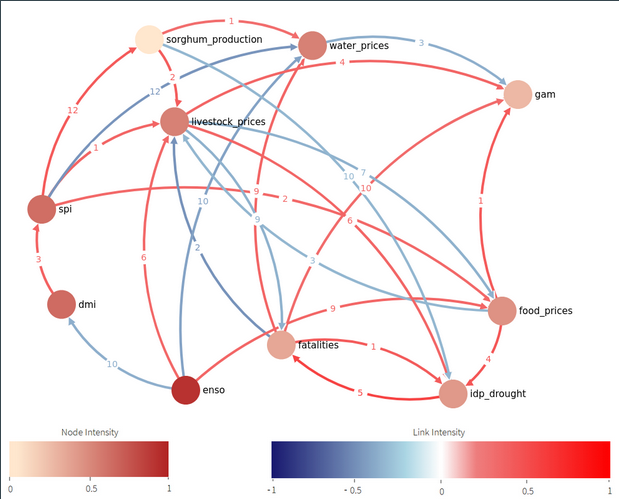
\includegraphics[scale=0.2]{images/baidoa}}
			\only<3>{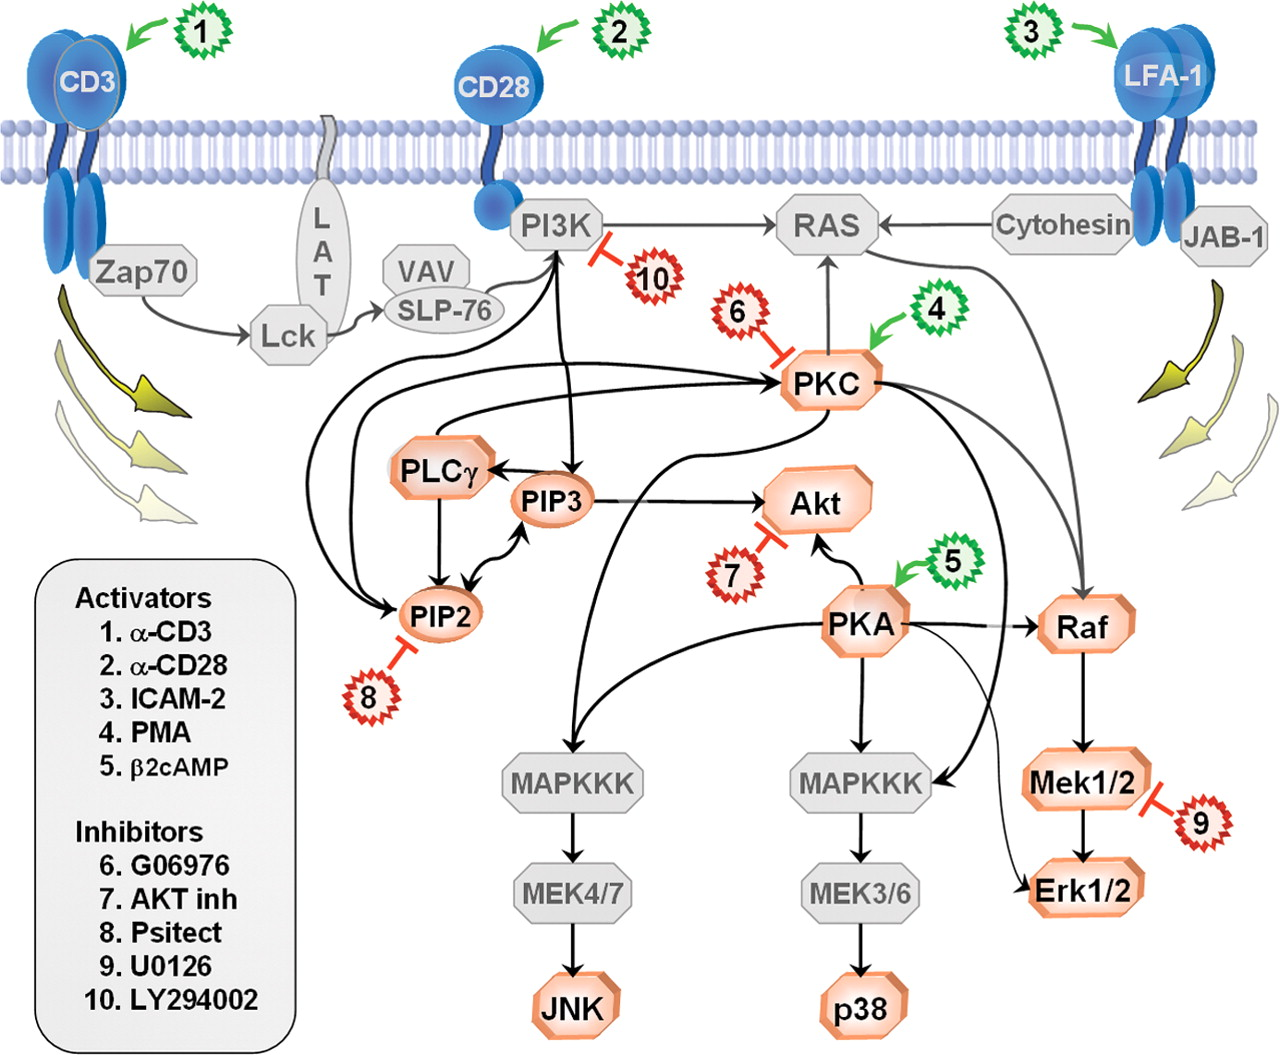
\includegraphics[scale=0.1]{images/grn}}
		\end{column}
	\end{columns}
\end{frame}

\begin{frame}{Causal Discovery} 
	\begin{itemize}
		\item<1-> Learn the structure/graph of the causal relationships between variables 
		\item<2-> If only two variables are considered: bivariate causal discovery 
		\item<3-> it always require assumptions 
		\item<4-> can use only observational data, or even interventions 
		\item<5-> usually the output is not a complete description of the causal relationships 
			  (depends on the assumptions, the type of data etc..) 
	\end{itemize}
\end{frame}

\begin{frame}{Causal Inference}
	\begin{columns}
		\begin{column}{0.5\textwidth}
			\begin{itemize}
				\item<1-> Estimate the strength of the effect of ENSO on vegetation 
					greenness
				\item<2-> How effective are humanitarian actions to fight food insecurity?  
				\item<3-> What is the effect of radiation on NEE/GPP ?  
					 Or the effect of temperature on RECO? 
			\end{itemize}
		\end{column}
		\begin{column}{0.5\textwidth}
			\only<1>{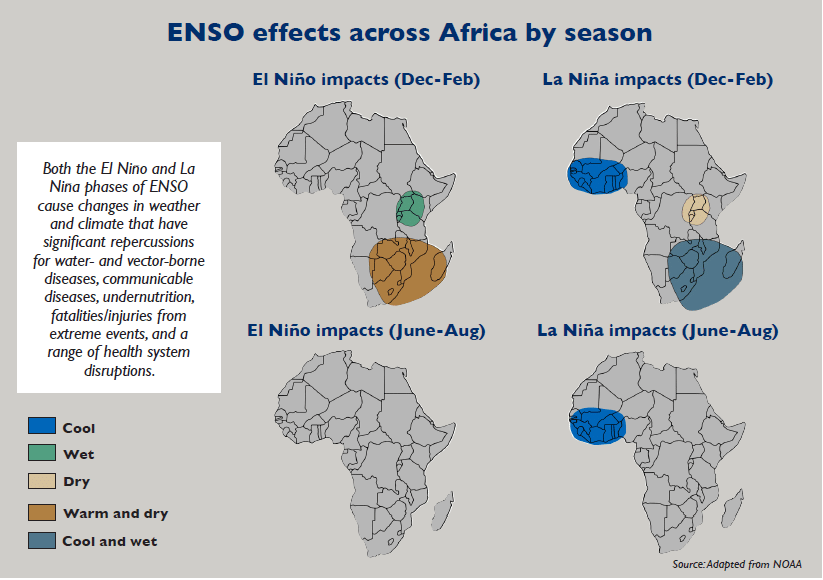
\includegraphics[scale=0.2]{images/Effects-of-ENSO-in-Africa}}
			\only<2>{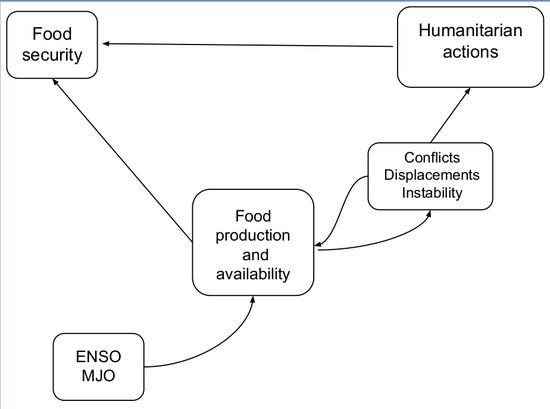
\includegraphics[scale=0.3]{images/foodaction}}
			\only<3>{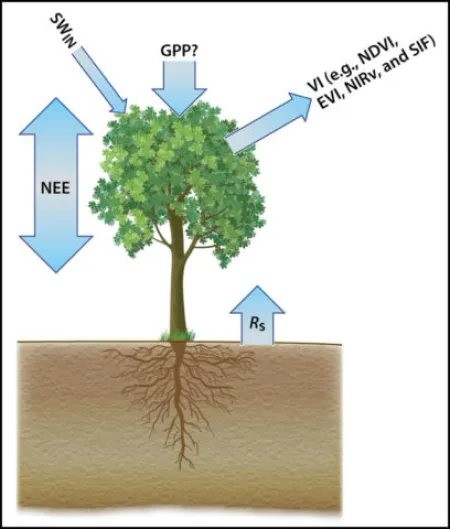
\includegraphics[scale=0.3]{images/nee}}
		\end{column}
	\end{columns}

\end{frame}

\begin{frame}{Causal Inference}
	\begin{itemize}
		\item  Estimate average treatment effect (ATE) or 
			conditional average treatment effect (CATE) 
		\item<2-> Usually provide confidence intervals and/or test hypothesis 
		\item<3-> Consider possible biases: confounding, selection biases, estimation biases  
	\end{itemize}
\end{frame}

\begin{frame}{Causal ML}
	\begin{itemize}
		\item Spurious relationships 
		\item Causal representation learning
		\item Causal feature extraction/ feature selection 
		\item robustness to intervention
		\item causal XAI 
		\item Causal RL 
	\end{itemize}
	\blfootnote{\citet{kaddour2022causal}}
´\end{frame}


\begin{frame}[allowframebreaks]
\bibliography{biblio}
\end{frame}

\end{document}


